\section{Experiment}
\label{sec:experiment}

We looked maximum a posteriori learning of the logistic regression classifier in class. In particular, we showed that learning the classifier is equivalent to the following optimization problem:
\[
\min_{\bw} \left\{\sum_{i=1}^m \log\P{1+ \exp(-y_i\bw^T\bx_i)} + \frac{1}{\sigma^2}\bw^T\bw\right\}
\]
In this question, you will derive the stochastic gradient descent algorithm for the logistic
regression classifier, and also implement it with cross-validation. Detailed instructions on cross-validation procedure can be found in homework 1, and instructions on SGD can be found in homework 4.

\begin{enumerate}
\item ~[5 points] What is the derivative of the function $\log\P{1+ \exp(-y_i\bw^T\bx_i)}$ with respect to the weight vector?

\begin{itemize}
\item We can simply treat $\mathbf{w}$ as a variable and it becomes a normal differentiation problem
\begin{align}
f(\mathbf{x}_{i}) &= \log\P{1+\exp(-y_{i}\mathbf{w}^{T}\mathbf{x}_{i})}\\
\intertext{where we can perform a $u$-substition such as}
u &= 1 + \exp\left(-y_{i}\mathbf{w}^{T}\mathbf{x}_{i}\right)\\
\frac{\text{d}u}{\text{d}\mathbf{w}^{T}} &= -y_{i}\mathbf{x}_{i}\exp\left(-y_{i}\mathbf{w}^{T}\mathbf{x}_{i}\right)\\
\intertext{such that we can use these to differentiate $f(\mathbf{x}_{i})$ to be}
\frac{\partial f(\mathbf{x}_{i})}{\partial \mathbf{w}^{T}} &= \frac{\partial f(u)}{\partial \mathbf{w}^{T}}\frac{\partial u}{\partial \mathbf{w}^{T}} = \frac{-y_{i}\mathbf{x}_{i}}{\exp\left(y_{i}\mathbf{w}^{T}\mathbf{x}_{i}\right)+1}\label{eq:expo}
\intertext{To overcome instances of {\em overflow errors} in the computations, this equation can be rewritten in the following (equivalent) format from when Equation~(\ref{eq:expo}) overflows}
\frac{\partial f(\mathbf{x}_{i})}{\partial \mathbf{w}^{T}} &= \frac{(-y_{i}\mathbf{x}_{i})\cdot \exp(-y_{i}\mathbf{w}^{T}\mathbf{x}_{i})}{1 + \exp(-y_{i}\mathbf{w}^{T}\mathbf{x}_{i})}
\end{align}
\end{itemize}


\item ~[5 points] The inner most step in the SGD algorithm is the gradient update where we use a single example instead of the entire dataset to compute the gradient. Write down the objective where the entire dataset is composed of a single example, say $(\bx_i, y_i)$. Derive the gradient of this objective with respect to the weight vector.

\begin{itemize}
\item We want the weight vector that minimizes our function, $J(\mathbf{w})$, so we need to take the gradient of it, but first we can {\em simplify} $J(\mathbf{w})$ to make the computation easier, which results in

\begin{align}
J(\mathbf{w}) &= \sum_{i=1}^{n}\log\P{1+\exp(-y_{i}\mathbf{w}^{T}\mathbf{x}_{i})}+\frac{\mathbf{w}^{T}\mathbf{w}}{\sigma^{2}}\\
&= \sum_{i=1}^{n}\log\P{1+\exp(-y_{i}\mathbf{w}^{T}\mathbf{x}_{i})}+\frac{\left|\left|\mathbf{w}\right|\right|^{2}}{\sigma^{2}}\\
\intertext{where we can take the derivative of this with respect to $\mathbf{w}$ and drop the summation since we're treating each record as the {\em only} data point. The first term is the same as the result in Equation~(\ref{eq:expo}) so only the second term needs to be differentiated with respect to $\mathbf{w}$.}
\frac{\partial J(\mathbf{w})}{\partial \mathbf{w}}&= \frac{-y_{1}\mathbf{x}_{1}}{\exp(y_{1}\mathbf{w}^{T}\mathbf{x}_{1})+1} + 2\frac{\left|\left|\mathbf{w}\right|\right|}{\sigma^{2}}\label{eq:grad-J}
\end{align}
\end{itemize}

\item ~[10 points] Write down the pseudo code for the stochastic gradient algorithm using the gradient from previous part.

\begin{itemize}
\item The pseudo code is represented in Algorithm~\ref{alg:SGD}, where $\gamma$ is the learning rate where $C=\sigma^{2}$, and there's a vector $\mathbf{x}_{i}\in\mathbb{R}^{n\times 1}$ in a set $S$ with $m$ different ``records.'' $t$ ranges from 1 to $(T\cdot m)$, where $T$ is the maximum number of epochs, since $\mathbf{w}$ isn't initialized to $\vec{0}$ at the start of each epoch.
\begin{algorithm} % enter the algorithm environment
\begin{algorithmic}% enter the algorithmic environment
\STATE Initialize $\mathbf{w}_{(0)}\in\mathbb{R}^{n\times 1}$
\STATE Initialize list $\mathbf{w}_{list}\in\mathbb{R}^{T\times n}$
\FOR{$epoch=1,2,\ldots\ $\TO $T$}
\FORALL{$(\mathbf{x}_{i},y_{i})\in S$}
\STATE{Pick random example $(\mathbf{x}_{i},y_{i})$}
%\STATE{$J\left(\mathbf{w}_{(t)}\right) = \frac{1}{2}\mathbf{w}_{(t)}^{T}\mathbf{w}_{(t)}+C\sum_{i=1}^{n}\max\left[ 0, 1-y_{i}\mathbf{w}_{(t)}^{T}\mathbf{x}_{i,t} \right]$}
\STATE{Treat $(\mathbf{x}_{i},y_{i})$ as a full dataset and compute $\Grad{J\left(\mathbf{w}_{(t)}\right)}$ from Equation~(\ref{eq:grad-J})}
\STATE{$\gamma_{(t)} = \frac{\gamma_{0}}{1+(\gamma_{0}\cdot t)/C}$}
\STATE{$\mathbf{w}_{(t+1)} = \mathbf{w}_{(t)} - \gamma_{(t)}\Grad{J\left(\mathbf{w}_{(t)}\right)}$}
\ENDFOR
\STATE Append $\mathbf{w}$ from current $epoch$ to $\mathbf{w}_{list}$
\ENDFOR
\RETURN{$\min_{\mathbf{w}\in\mathbf{w}_{list}}\left\{ \sum_{i=1}^m \log\P{1+ \exp(-y_i\bw^T\bx_i)} + \frac{\left|\left|\mathbf{w}\right|\right|^{2}}{\sigma^2}  \right\}$}
\end{algorithmic}
\caption{Stochastic Gradient Descent$(S=\{(\mathbf{x}_{i},y_{i})\}_{m})$}
\label{alg:SGD}
\end{algorithm}
\end{itemize}


\item ~[20 points] Implement your pseduo code as a training algorithm with
  cross-validation on the $\sigma$ parameter.  This parameter
  basically helps trade off between generalizability and model fit.  

  Use the two {\tt astro} data sets (original and scaled) from
  homework 4 to train and evaluate the learner. In your writeup,
  please report on the accuracy of your system, what value of sigma
  you chose based on cross validation, how many epochs you chose to
  run SGD, and a plot of the NEGATIVE log likelihood after each epoch
  of SGD. %

\begin{itemize}
\item In order to implement Stochastic Gradient Descent, Algorithm~\ref{alg:SGD} was used. In doing so, there was a hyper parameter $\sigma$ which needed to be chosen. However, the ``learning rate'' $\gamma_{(t)}$ was dependent upon an initial value, $\gamma_{0}$, and some parameter $C$ where $C=\sigma^{2}$. This learning rate changed over time and was defined as $\frac{\gamma_{0}}{1+(\gamma_{0}\cdot t)/C}$ which was important as the learning rate would decrease over time as the function presumably as it approached the maxima. These hyper parameters were {\em also} used to get the general range of what they should be. Table~\ref{table:hp_range} indicates the ranges that were initially trained over to see what the best values to use were. In the table, it only lists the minimum and maximum values, though the intermediary values were powers of 10 between the min and max. 

\begin{table}[!h]
\centering
\begin{tabular}{c | c c}
\hline\hline
{\bf Parameter} & {\bf Min} & {\bf Max}\\
\hline
$\sigma$ & $10^{-7}$ & $10^{3}$\\
$\gamma_{0}$ & $10^{-10}$ & $10^{-3}$\\
\hline
\end{tabular}
\caption{Hyper-parameter Cross Validation Ranges}
\label{table:hp_range}
\end{table}

Using these ranges, 5-fold cross validation was implemented on the training data to get the best parameters for the model. Table~\ref{table:acc_orig} shows the top 5 parameters for the file \verb~astro/original/train~ while Table~\ref{table:acc_scaled} shows the top 5 parameters for the file \verb~astro/scaled/train~. The {\em best} value was chosen for each file, which was then used to train over the {\em entire} training set and then used to classify the test data. During Cross Validation, only 5 epochs were chosen and it was only 5-fold cross validation

\begin{table}[!h]
\centering
\begin{tabular}{c c c c}
\hline\hline
{\bf Accuracy} & $\boldsymbol{\gamma_{0}}$ &  $\boldsymbol{\sigma}$\\
\hline
$0.91229$ & $10^{-7}$ &  $100$\\
$0.91196$ & $10^{-7}$ &  $10$\\
$0.91196$ & $10^{-7}$ &  $0.1$\\
$0.91164$ & $10^{-7}$ &  $1000$\\
$0.91099$ & $10^{-7}$ &  $1.00$\\
\hline
\end{tabular}
\caption{Top 5 hyper-parameter combinations for {\tt astro/original/train}}
\label{table:acc_orig}
\end{table}

\begin{table}[!h]
\centering
\begin{tabular}{c c c c}
\hline\hline
{\bf Accuracy} & $\boldsymbol{\gamma_{0}}$ & $\boldsymbol{\sigma}$\\
\hline
$0.54298$ & $10^{-8}$ &  $0.001$\\
$0.54298$ & $10^{-8}$ &  $0.001$\\
$0.54298$ & $10^{-8}$ &  $0.001$\\
$0.54298$ & $10^{-7}$ &  $0.001$\\
$0.54298$ & $10^{-6}$ &  $0.001$\\
\hline
\end{tabular}
\caption{Top 5 hyper-parameter combinations for {\tt astro/scaled/train}}
\label{table:acc_scaled}
\end{table}


As can be seen in the tables, in the original data $\sigma$ varied while the other parameters stayed the same. The opposite was true for the scaled data, where $\sigma$ remained constant and the other parameters varied. From using the best hyper-parameters, where 10 epochs for each data set was chosen. The test set \verb~astro/original/test~ scored a classification accuracy of $0.90625$, while the scaled data did much worse and \verb~astro/scaled/test~ had a classification accuracy of $0.50000$. These results agree pretty well with the last homework assignment which is reassuring on the implemented algorithm working correctly. Figure~\ref{fig:neg_loger} shows the negative log likelihood function of each of the test files at the end of each epoch.

\begin{figure}[!h]
\centering
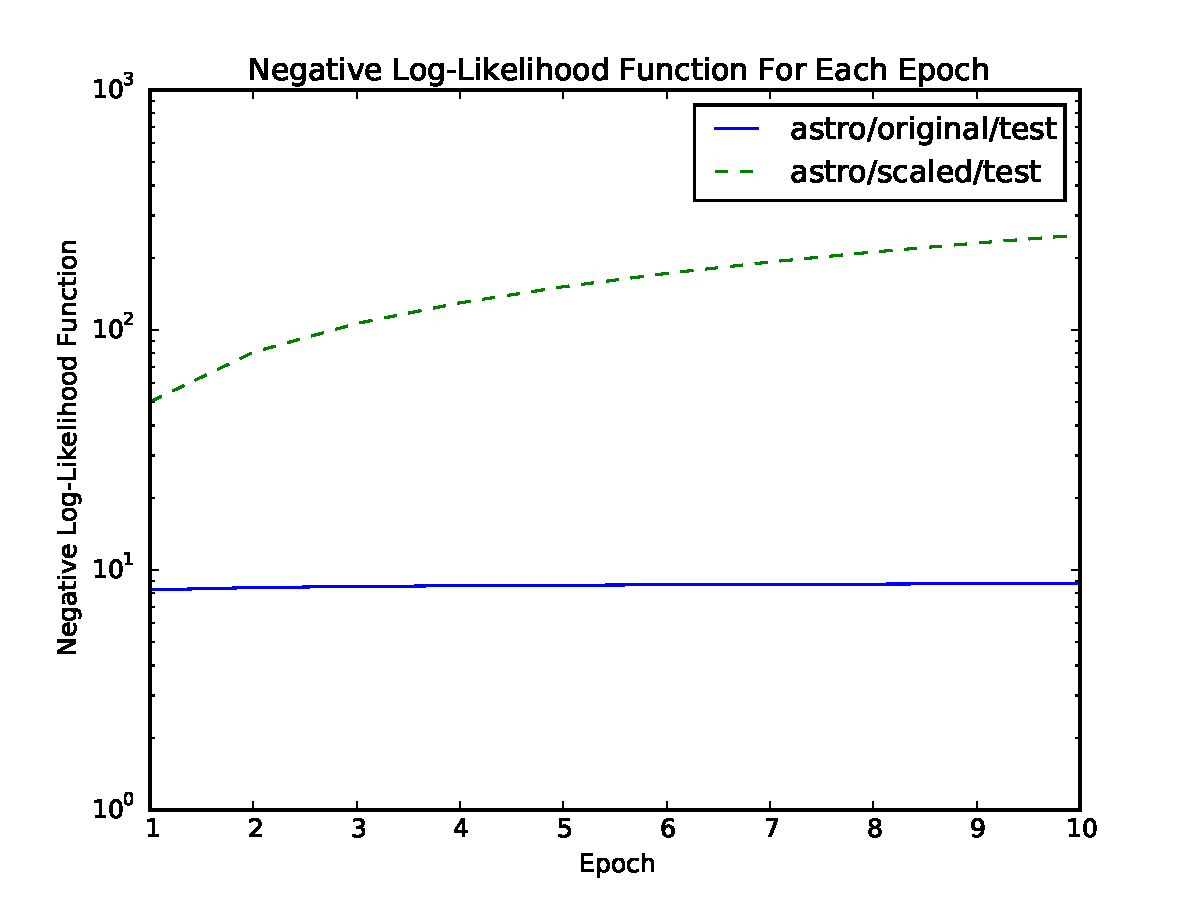
\includegraphics[width=.65\textwidth]{SGD-results_final.pdf}
\label{fig:neg_loger}
\caption{Negative Log Likelihood Function of $J(\mathbf{w})$}
\end{figure}
\end{itemize}


\end{enumerate}

{\bf As mentioned in previous homeworks, you may use any programming
  language for your implementation. Upload your code along with a
  script so the TAs can run your solution in the CADE environment}.



%%% Local Variables:
%%% mode: latex
%%% TeX-master: "hw5"
%%% End:


%%% Local Variables:
%%% mode: latex
%%% TeX-master: "hw5"
%%% End:
